
\documentclass[12pt]{article}
\usepackage[utf8]{inputenc}
\usepackage[a4paper]{geometry}
\usepackage{amsmath}
\usepackage{amsfonts}
\usepackage{amssymb}
\usepackage{natbib}
\usepackage[english]{babel}
\usepackage{listing}
\usepackage{textgreek}
\usepackage[xllnames]{xcolor}
\usepackage[colorlinks=true,citecolor=blue]{hyperref}
\usepackage{blindtext}
\usepackage{graphicx}
\usepackage{listings}
\usepackage[ruled,vlined,linesnumbered]{algorithm2e}
\renewcommand{\baselinestretch}{1.5}

\geometry{hscale=0.85,vscale = 0.90,centering}

\title{Automated seqFISH data analysis : Mathematical Appendix}
\author{Pierre Bost, Uria Mor, Florian Mueller}

\begin{document}


\maketitle

{
  \hypersetup{linkcolor=black}
  \tableofcontents
}
\newpage


\section{SeqFISH data : properties and challenges}


\subsection{Introduction}

SeqFISH \citep{shah_situ_2016,eng_transcriptome-scale_2019}, and other similar techniques such as osmFISH \citep{codeluppi_spatial_2018}, and MERFISH \citep{chen_spatially_2015} generate large amount of raw data in the form of high resolution (100x) multi-stacks (20-50) microscopy images. While whole organs are usually not imaged, large regions of several mm2 are typically studied generating up to Terabytes of data. Those data usually consist in .Tiff files that cannot be directly used and  have to be pre-processed similarly to the raw .fastq files that have to be heavily processed to generate gene count tables.

While the protocol is supposed to generate clean image with high Signal to Noise Ratio (SNR), we observed in practice significant background signal, as well as non specific binding of the probes making the analysis of such data extremely complex. In the following part of the manuscript we will describe what are the different steps of the pipelines as well as the mathematical foundation on which our pipeline relies on.

\subsection{Automated processing of seqFISH data is required}

The most common use of seqFISH raw data consist in converting them into tables containing the location of each identified cell together with their gene expression level. This requires two key steps : spot detection and cell segmentation. While both tasks can be performed manually for small datasets generated by smFISH technology, this is not feasible for seqFISH data primarily due to the large number of genes studied (up to hundreds in some experiments). Moreover as the data need to be analyzed in a robust and reproducible manner, human intervention need to be as limited as possible. Indeed manual image analysis methods tends to  :
\begin{itemize}
\item Be poorly reproducible.
\item Be tedious and time-consuming while finding an appropriate cut-off values.
\item Exhibit high intra- and inter-user variability.
\end{itemize}
Therefore fully automated seqFISH raw data processing is required.

\subsection{Current state of the art}

To our knowledge no freely available pipeline dedicated to seqFISH has been developed : indeed each paper using seqFISH-like data tend to use a specific script. While those scripts are freely available, they lack clear documentation and robust mathematical foundations that would make them broadly usable and applicable. In addition, many scripts do not address the issue of efficient and robust cell segmentation as well as non specific probe binding.

On the other hand, efficient tools have been developed for smFISH data such as FISH-quant \citep{mueller_fish-quant:_2013} but are relying on a user defined threshold and are not designed to deal with large datasets. Furthermore, cell segmentation is also performed manually or is only automated in case of in-vitro data.
Therefore there is a need for a simple, robust and yet computationally efficient method for seqFISH data pre-processing.

\section{Detection and counting of RNA molecules}

\subsection{Choice of the method}

Spot detection is the first and most important step of seqFISH data processing. As we did not aim to create a new spot detection algorithm but rather identify the most suited approach, we screened recent review\citep{ruusuvuori_evaluation_2010,smal_quantitative_2010,stepka_performance_2015} and looked for a method with little to no false positive, robust to background noise and with easily understandable parameters. We identified the H-Dome (HD) and the Multiscale methods as the most efficient and adapted method \citep{smal_quantitative_2010,stepka_performance_2015}, each of them having specific advantages and drawbacks.

The following part of the subsection will be devoted to the description of the mathematical background of the HD and Multiscale method as well their respective software implementation. If not stated otherwise, all functions used are Matlab® functions.

\subsection{H-dome based spot detection}

We selected the HD method because :
\begin{enumerate}
\item It has the highest accuracy (F-score) for small object detection.
\item Overall it has the best performance independently of the object shape when the hypothesis made (given size and circular shape) are met.
\item Key parameters of the HD method correspond to precise features of the RNA spots (minimal and maximal size, estimated SNR).
\end{enumerate}

However HD suffers from high computational cost and strong sensitivity to the parameters, therefore requiring careful parameter tuning so that it will perform reasonably across all channels and images. 


\subsubsection{LoG filter}

As all spot/small object detection methods, HD method relies on three successive steps : noise reduction, signal enhancement and signal thresholding.
In our case, noise reduction and signal enhancement is performed simultaneously by applying Laplacian of Gaussian (LoG) filter on the image \citep{sponton_review_2015}. The LoG filter consists in first applying a Gaussian convolution filter G and then computing the Laplacian value at each pixel \citep{sponton_review_2015}. Such filter is commonly used in many image analysis cases, such as edge and blob/spot detection and has already been used for RNA spot detection for smFISH data \citep{mueller_fish-quant:_2013}.

More formaly, lets $I(x,y)$ be the intensity of the Image of interest at location $(x,y)$. Applying Gaussian kernel consist in computing the convolution product of the Image and and a function $G_{\sigma}$ :
\begin{equation}
G_{\sigma}(x,y) = \frac{1}{\sqrt{2 \pi \sigma^2}} e^{-\frac{x^2+y^2}{2\sigma^2}}
\end{equation} 

The resulting image $g(x,y)$ is therefore :
\begin{equation}
g(x,y) = G_{\sigma}(x,y)*I(x,y)
\end{equation}

where $*$ corresponds to the convolution product.
The final image $L(x,y)$ is obtained by applying Laplacian operator :

\begin{equation}
L(x,y) = \nabla^2(G_{\sigma}(x,y)*I(x,y))
\end{equation}
This can be simplified as :

\begin{align}
L(x,y) & = (\nabla^2G_{\sigma}(x,y))*I(x,y) \\
& = LoG_{\sigma}*I(x,y)  \nonumber
\end{align}

It is therefore enough to convolute the original image with the $LoG_{\sigma}$ function :
\begin{equation}
LoG_{\sigma}(x,y) =  \frac{x^2+y^2-2\sigma^2}{\sigma^4}e^{-\frac{x^2+y^2}{2\sigma^2}}
\end{equation}
Such function is often called the 'Mexican hat' due to it shape (ref Figure plot Log function) and is implemented using the imfilter and fspecial functions.

\begin{figure}[!h]
	\begin{center}
		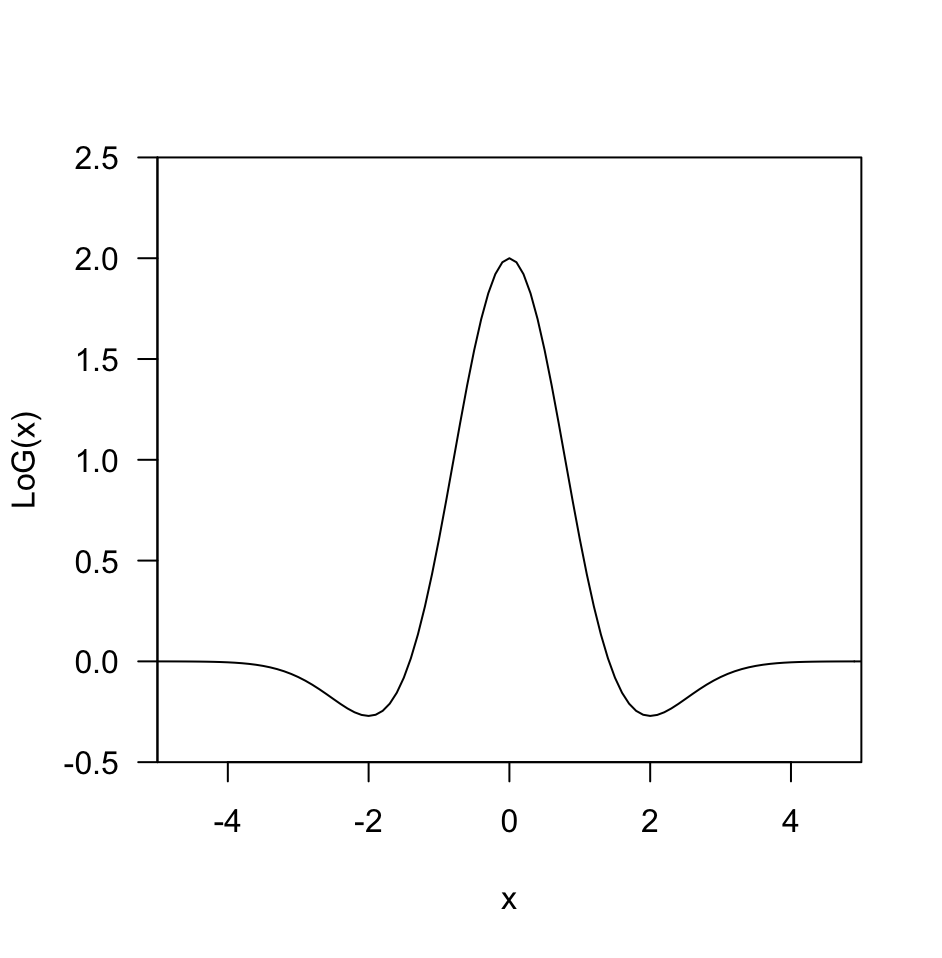
\includegraphics[width=0.5\linewidth]{LoG_function.png}
		\caption{Laplacian of Gaussian (LoG) function value}
		\label{Fig:Log}
	\end{center}
\end{figure}

In practice we add to small steps :
\begin{itemize}
\item Taking the opposite of the transformed image so that the highest values correspond to local maximum and not local minimum.
\item Sizing the values of transformed image between 0 and 1 (imadjust function).
\end{itemize}

The choice of the parameter $\sigma$ is essential for the whole spot detection analysis : if it too small the image will not be smoothed enough and noise will be considered as spot while if it is too large spots will be considered as noise and removed. Typically $\sigma$ value will correspond to the radius of a spot (one or two pixels). In the following part of the manuscript this parameter will be name $\sigma_{small}$.

\subsubsection{H-dome transformation}

The next step consist in identifying and extracting the local maxima of a given height. To do so we use a method based on morphological grayscale reconstruction : the h-dome transform. As we do not aim to describe the whole field of morphological grayscale reconstruction we recommend to the reader the field founding paper by Luc Vincent \citep{vincent_morphological_1993}.

The h-dome transform aims to identify the so called h-dome structure which are defined as follow. Lets $D$ be a set of connected/neighbor pixels and $h$ a strictly positive real number. Then it is an h-dome if and only if :
\begin{itemize}
\item Every pixel $p$ neighbor of $D$ satisfies $I(p) < \min\{ I(q) | q \in D \}$, i.e it is a local maximum.
\item  $\max\{ I(q) | q \in D \} -\min\{ I(q) | q \in D \}  < h $, i.e the difference of intensity between the brightest and dimmest pixel is lower than $h$.
\end{itemize}
where $I(p)$ corresponds to the pixel intensity of the pixel $p$.

 
\begin{figure}[!h]
	\begin{center}
		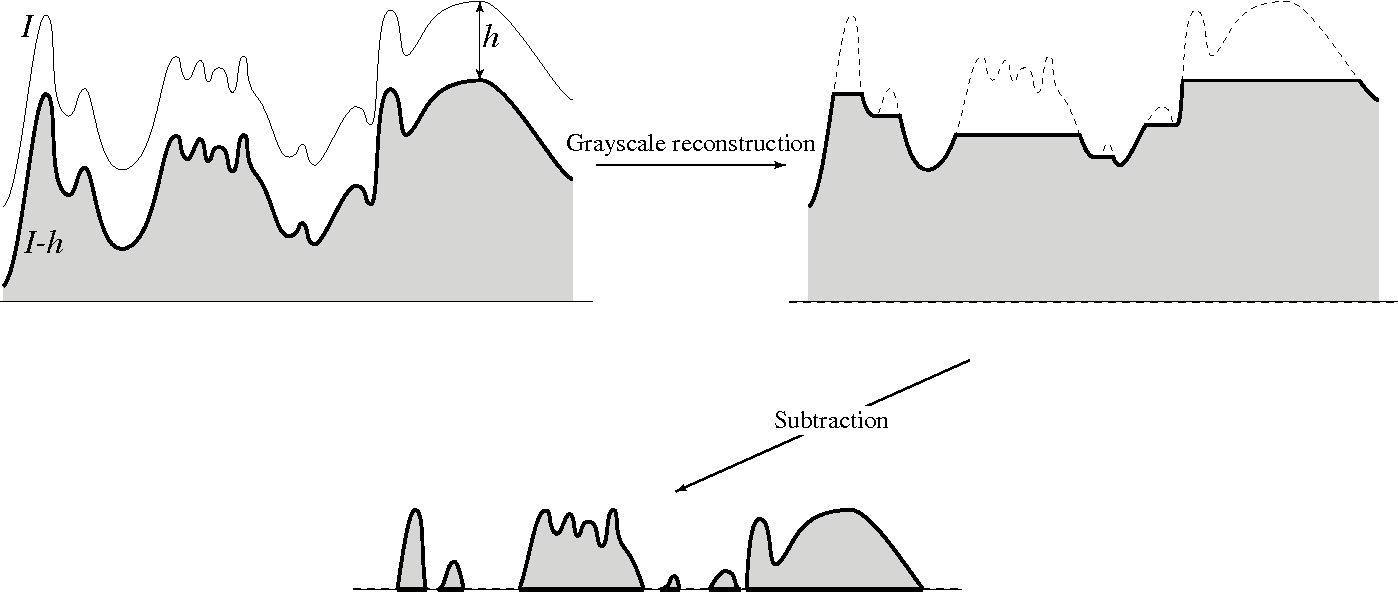
\includegraphics[width=1\linewidth]{H_dome.png}
		\caption{Example of the H-dome transform (from \citep{vincent_morphological_1993}).}
		\label{Fig:H_dome}
	\end{center}
\end{figure}
 



Unlike classical top-hat transformation, the h-dome transformations isolates local maxima without involving any shape size or shape  but only height criterion. Interestingly resulting image only contains peaks of maximum height $h$.
The h-dome transformed image is generated using the imhmax function and will be called $M$ in the manuscript. 

The $h$ parameter need to be carefully chosen as a variation of it can dramatically change the result of the h-dome transform and hence of the whole spot detection analysis. To make the analysis more robust we used the following strategy : for each channel/gene we compute the mean and max value of the LoG transformed image $L(x,y)$ and use them to compute the $h$ parameter :

\begin{equation}
h = Std(L(x,y)) \times h_{Meta}
\end{equation}
where $h_{Meta}$ is a positive real number and $Std(L(x,y))$  the standard deviation of the $L(x,y)$ image.
The $h_{Meta}$ parameter need to be chosen : if the Signal to Noise Ratio (SNR) is expected to be high then $h$ has to be high and  $h_{Meta}$ also so that only the tip of the peak is selected while if the SNR is low then $h$ need to high enough to select real peaks.

\subsubsection{Pixel sampling and aggregation}

The filtered image is first transformed by raising the image values to a power $S$ and then by dividing each element by the total image intensity.

\begin{equation}
M_{normalised}(x,y)= \frac{M(x,y)^S}{\sum_{x=1}^{x_{max}} \sum_{y=1}^{y_{max}} M(x,y)^S}	
\end{equation}
where $x_{max}$ and $y_{max}$ correspond to the width and height of the image. Such transformation will favor strong signal and remove low intensity peaks. 

It is obvious that :
\begin{equation}
\sum_{x=1}^{x_{max}} \sum_{y=1}^{y_{max}} M_{normalised}(x,y) = 1
\end{equation}
Therefore the transformed image can be considered as a probability vector and we can sample pixels according to it. We therefore sample $N_{Sampled \; pixels}$ pixels according to this probability . 

The last step consist in aggregating the sampled pixels into spots. To do so the Mean-Shift (MS) algorithm is used. Briefly the MS algorithm identifies clusters as high density regions through an efficient hill-climbing algorithm based on kernel density estimator. In opposition to many other clustering techniques, the number of clusters does not need to be provided, making it particularly suited for our use case as we ignore the number of spots.  For more details we recommend the reader to look at the exhaustive and excellent review from Carreira-Perpinan \citep{carreira-perpinan_review_2015}.

 While efficient and well-suited , the MS algorithm suffers from two main issues :
\begin{enumerate}
\item It relies on a key parameter $w$ that controls the width of the kernel window used for density estimation.
\item It requires large CPU and memory  for big datasets (the kernel density estimator uses all the points at each iteration in its naive implementation)
\end{enumerate}

While the first problem can be easily solved as we expect the spot to have a precise size (empirically we used $w = 2\sigma_{small}$) the second problem requires to implement a modified version of the algorithm where at each iteration only the neighboring points that are close enough are used for the mean-shift computation. To do so, only points for which the corresponding weight after applying gaussian kernel  is bigger than 0.001 are used.  As this correspond to a Fixed-radius near neighbors finding, this can be efficiently performed through the use of K-D Tree and hence considerably reduces computational time. 

At the end of the MS algorithm we got a list of cluster centroids/positions as well as the pixels associated with it.

\subsubsection{Pixel clusters filtering}

The MS algorithm can produce spurious pixel clusters that do not correspond to real spots. Those pseudo-spots will tend to have few pixels or to be highly spread. Such criteria can be used to remove them. Let $C_{i}$ be the set of pixels associated with cluster i and $N_{Clusters}$ be the total number of clusters. Then :

\begin{equation}
\forall i \in [[1,N_{Clusters}]] \;  \;   \; C_{i} = \{P_{j} | Cluster(P_{j})=i \}
\end{equation}
where $P_{j}$ corresponds to the (x,y) position of pixel $j$.

We can them compute the number of pixels $Nc_{i}$  and the dispersion $Disp_{i}$ of  each pixel cluster~ $C_{i}$:

\begin{equation}
 Nc_{i} = |C_{i}|
\end{equation}
\begin{equation}
Disp_{i} = det(cov(C_{i}))
\end{equation}
where $cov(C_{i})$ corresponds to the empirical covariance matrix of pixel location belonging to cluster~ $i$.

We only kept clusters $i$ such that $Nc_{i} >5$ and $Disp_{i} < \sigma_{Max}^4$ where $\sigma_{Max}$ correspond to maximal size of the spot. This last filtering can be interpreted as follow : the size of a spot will be proportional to the determinant of the co-variance spot matrix. Therefore in the case of a purely spherical spot of characteristic size $\sigma$, the determinant of the matrix is therefore equal to $\sigma^2 \times \sigma^2 + 0 \times 0 = \sigma^4$.
The pixel clusters that pass those filtering are  considered as real spots and are then kept for further analysis.

\subsubsection{Parameters of the HD approach}

The HD relies on many different parameters  :
\begin{itemize}
\item The minimal spot size ($\sigma_{small}$)
\item The maximal spot size ($\sigma_{max}$)
\item The height of the extracted h-domes  ($h_{Meta}$)
\item The power to which the H-dome matrix is raised ($S$)
\item The number of pixels sampled ($N_{Sampled \; pixels}$)
\end{itemize}

While the HD method is highly efficient, it requires a fine tuning to be efficient in the case of low SNR. While $\sigma_{small}$ and $\sigma_{max}$ are easy to interpret and to tune, the $h_{Meta}$ and $S$ are way harsher to deal with, as both parameters strongly interact together. Lastly, the  $N_{Sampled \; pixels}$ parameter need to high enough to catch all the spots. However, in the case of highly genes (thousands of spots per image), we observed that the maximal number of pixels sampled (more than hundred thousands) can saturate the working memory, making the HD method not usable in that case.


\subsection{Multiscale spot detection}

While in case of simulated data, HD method performs best, it may suffer from a significant loss of accuracy in case of real data. Conversely, the Multiscale method exhibits highly robust performance and is easy to tune with lower performance in the case of low quality signal. We present here a modification of the original method published in \citep{foltankova_hybrid_2013}. If the reader is interested by a more comprehensive description of mathematical background on which the Multiscale approach is founded on, we recommend to read \citep{jin_vascular_2013}.


\subsubsection{Multiscale Hessian matrix determinant computation}

The first step of the Multiscale method consists in smoothing the original image with gaussian kernels of various size. Let $\sigma_{0}$ be the smallest $\sigma$ gaussian kernel parameter used and $N$ the number of different gaussian kernels used, we defined $\theta = \{\sigma_{i}\})_{k=0}^{N-1}$ where $\sigma_{k} =2^{k} \sigma_{0}$. For each different $\sigma_{k}$ we can therefore compute :

\begin{equation}
g_{k}(x,y) = G_{\sigma_{k}} * I(x,y)
\end{equation}

For each voxel of the smoothed image $g_{k}$, the Hessian matrix is then  computed :

\begin{equation}
H_{k}(x_{0},y_{0}) = \begin{bmatrix}
\frac{\partial^2 g_{k}}{\partial x^2} & \frac{\partial^2 g_{k}}{\partial x \partial y} \\
\frac{\partial^2 g_{k}}{\partial y \partial x} & \frac{\partial^2 g_{k}}{\partial y^2} \\
\end{bmatrix}_{(x_{0},y_{0})}
\end{equation}

In practice, the Hessian matrix components are computed using the Sobel operator. The determinant of the Hessian matrix is then used to estimate the total signal variation. Therefore a new image can be computed for each $sigma_{k}$ value :

\begin{equation}
V_{k}(x,y) = det(H_{k}(x,y))
\end{equation}

Finally by taking for each pixel the maximal value across all $V_{k}$ images, we obtained a new image $M$ that highlights local variations at several scales, making the spot detection step more robust.

\begin{equation}
M(x,y) = \max_{k}(V_{k}(x,y))
\end{equation}

\subsubsection{Automated thresholding and spot extraction}

The obtained $M$ matrix is then automatically thresholded using the triangle's method. Briefly the triangle method consists in selecting the point in the image intensity histogram that maximize the distance with the diagonal line of the height and range and then adding a fixed offset $T_{offset}$ \citep{zack_automatic_1977}.  

 
\begin{figure}[!h]
	\begin{center}
		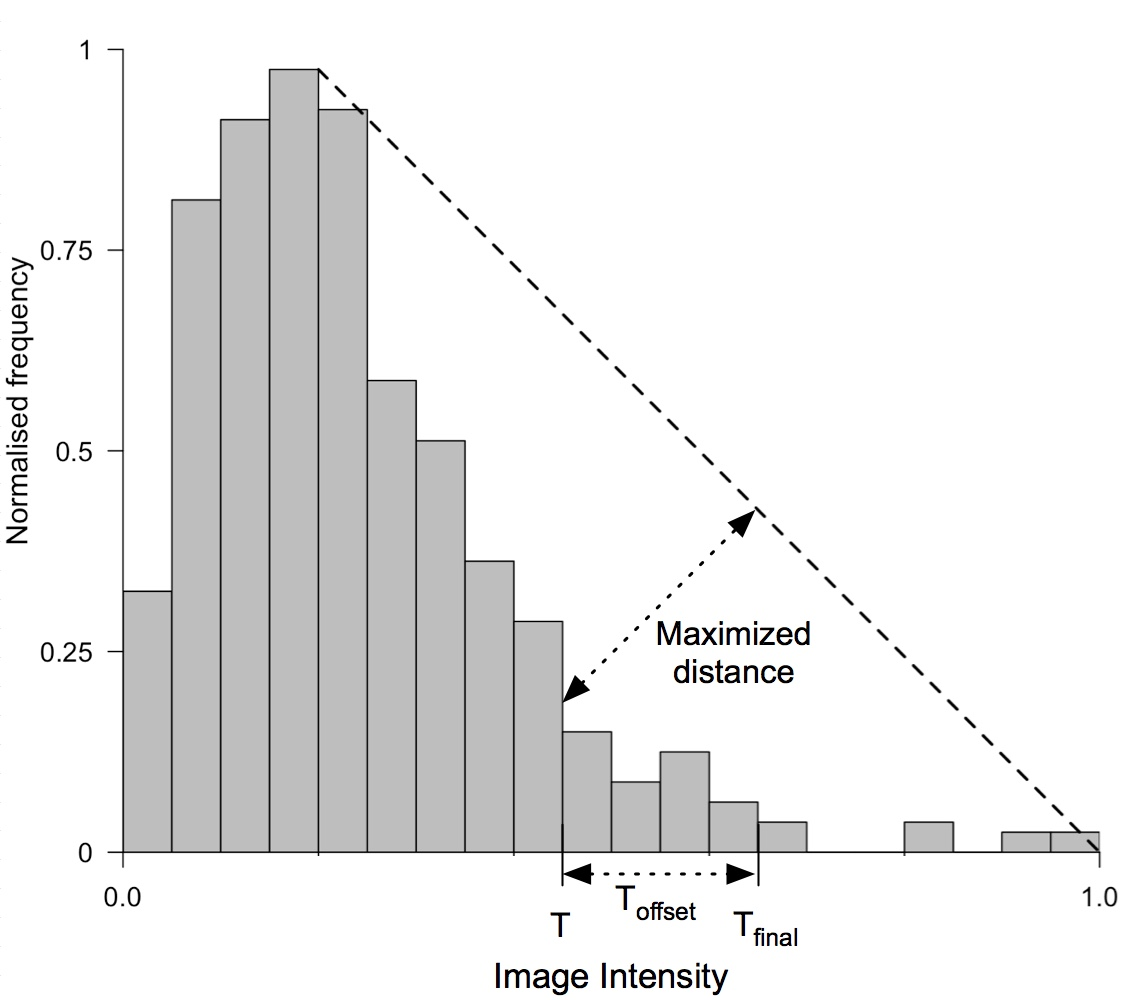
\includegraphics[width=0.7\linewidth]{Triangle_binarisation.jpeg}
		\caption{Description of the triangle binarization method}
		\label{Fig:Triangle_method}
	\end{center}
\end{figure}
 
The connected components of the thresholded images are then extracted and their centroid used as spot location. Connected components with more than 5 pixels are kept and considered as spots.

\subsubsection{Parameters of the Multiscale approach}

In conclusion, the Multiscale approach relies on three different parameters : $\sigma_{0}$ (minimal smoothing parameter), $N$ (number of scales) and $T_{offset}$ (offset to threshold used in the binarisation step). The first two parameters are easy to tune as   $\sigma_{0}$ can be set to the minimal size of a spot (at least one pixel) and and $N$ should simply be above a given value to avoid missing larger objects. We however recommend not to use a too high value of $N$ that would significantly increases computation time. Lastly the $T_{offset}$  parameter can be used to fine tune the thresholding step but is by default set to 0 to avoid over-fitting and increase robustness of the analysis.


\subsection{Removing non specific spots}

While the HD and Multiscale method are extremely efficient at identifying spots, they can still be fooled by a specific type of technical artifact : the non-specific  binding of  probes and of HCR amplifiers to sub-cellular structures. This can generate false positive signal and artificial spots that have no biological meanings.
To remove such artifacts we used the following empirical observations :
\begin{itemize}
\item Those spots are dimmer than the real RNA spots.
\item They are spread uniformly across the tissue while the real spots are highly clustered. 
\end{itemize}

We therefore used a spatial clustering based approach :
\begin{enumerate}
\item First the image intensity at each spot location is extracted.
\item The local spot density is computed using the density.ppp function from the R package spatstat.
\item For 30 different intensity threshold, the spots with an intensity below the value are removed and a Kulldorf's spatial scan test is computed \citep{kulldorff_spatial_1997}. The corresponding Likelyhood Ratio ($LR$) is then extracted.
\item The intensity with the highest $LR$ is selected and all spots with an intensity below this threshold are considered as noise and removed.
\end{enumerate}

The Kulldorf's spatial test consists in checking if there is at least one zone of the image where the spot density is not coherent with a background spatial distribution, in our case an non-homogeneous Poisson Point Process (PPP) derived from the initial spot distribution. More details can be found in Kulldorf's paper \citep{kulldorff_spatial_1997}.

\subsection{Quality Control of the spots}

Now that the points have been identified and filtered, the Quality Control of the spot analysis can be performed. To provide as much information as possible to the user the following features are displayed for each position and each channel/gene :
\begin{itemize}
\item The number of spots identified before and after filtering.
\item The ratio of spots that pass or not the filtering.
\item The mean Signal to Noise Ratio (SNR) of the spot.
\end{itemize}

For each spot $i$, its SNR ($SNR_{i}$) is computed by extracting the neighbor pixel intensity (a square box of seven pixel width and height is used) and estimating the corresponding standard variation $\sigma_{i}$. If the itensity of the spot is $\mu_{i}$, then its SNR  is simply :
\begin{equation}
SNR_{i} = \frac{\mu_{i}}{\sigma_{i}}
\end{equation}

We consider that below a mean SNR of 2, a channel should not be used and that the identified spots are mostly noise. Similarly, a mean SNR above 5 correspond to a high quality channel and can be used without any risk for further analysis.


\section{Cell segmentation}

\subsection{Limitations of current cell segmentation methods}

Cell segmentation is an essential step for automated microscopy image processing that allows to quantify a given measurement/feature (RNA or protein expression) at a single-cell resolution. While fully automated cell segmentation is easily performed on in-vitro cell images, doing it on in-vivo cell images remain challenging. 
Numerous  experimental and computational strategies have already been developed but all of present significant drawbacks that limit their use in seqFISH technology :
\begin{itemize}
\item DAPI/nuclear based techniques can not be used if the cells are not rounds or if the tissue is too crowded such as in lymphoid tissues.
\item Membrane staining through antibody or Wheat Germ Agglutinin (WGA) is not compatible with some seqFISH protocols that use SDS for tissue cleaning.
\item Cytoplasm staining, such as the Nissl staining, has already been used with seqFISH \citep{shah_situ_2016} but requires manual analysis due to high cell crowding. 
\item Background signal based segmentation, a powerful strategy already used for in-vitro smFISH image analysis can not be used on tissues samples as the background can be generated by non cellular structures \citep{mueller_fish-quant:_2013}.
\end{itemize}

There is therefore a need for an automated cell segmentation method that could be apply on any seqFISH dataset, independently of the imaged tissue structure and underlying cells shape. 

\subsection{RNA spots based segmentation}


\subsubsection{Principles}

Our segmentation method is based on the following empiric observation : genes that are highly expressed but only in a limited set of cells can be used ton infer the shape the cells. Indeed if a gene is highly expressed by a cell, its RNA molecules will usually spread across its whole cytoplasm, revealing the cell shape. Moreover, if only a minor fraction of the cells express that gene, the probability that two touching cells express that gene is low and therefore the observed structures will not originate from two neighbor cells.
We thus developed an automated cell segmentation method based on this observation. This method relies on the following steps :
\begin{enumerate}
\item For each gene, the spots are clustered using a spectral based approach, inspired from the improved NJW clustering algorithm and from the Diffusion Map dimensionality reduction method\citep{ng_spectral_2001,zelnik-manor_self-tuning_2004,nadler_diffusion_2005}.
\item The obtained clusters are filtered out to remove spurious clusters. Clusters obtained across all genes are then compared and overlapping clusters are aggregated
\item For each cluster aggregate, the associated spots are used to compute the final shape of the cell.  
\end{enumerate}

\subsubsection{Spectral clustering of the RNA spots}

To cluster the RNA spots in a shape and cluster number agnostic way, we decided to use a method inspired from the NJW clustering approach \citep{ng_spectral_2001,zelnik-manor_self-tuning_2004} and from the diffusion map dimensionality reduction tool. Both methods are highly linked and an extensive comparison can be read in \citep{nadler_diffusion_2005}.

Our clustering approach starts by computing the similarity between all $n$ RNA spots of a given gene at a given position. Let $x_{i}$ and $x_{j}$ be the location of points $i$ and $j$ respectively. We define the similarity $s(i,j)$ between those two points as :
\begin{equation}
s(i,j) = \exp(\frac{-d(x_{i},x_{j})^2}{2\sigma_{i}\sigma_{j}})
\end{equation}
where $d(x_{i},x_{j})$ corresponds to the euclidean distance between points $i$ and $j$, while $\sigma_{i}$ and $\sigma_{j}$ correspond to the distance of point $i$ (and $j$ respectively) to their $K$ nearest neighbor. Typically $K$ value will be around 10/20. Such approach avoid to manually define a global $\sigma$ value and to deal with varying point density in the sample space.

The similarity matrix $S$, defined by $S_{i,j} = s(i,j)$, is then normalized to produce a stochastic matrix :

\begin{equation}
M = D^{-1}S
\end{equation}
where $D$ is a diagonal normalization matrix with $D_{i,j}=\sum_{j}S_{ij}$ . We now can utilize the fact that by construction M is stochastic matrix with rows summing to one and can be thus interpreted as a transition matrix and defines a random walk. Under this view $M_{i,j}$ defines the transition probability between points $i$ an $j$ in one step.

 We can therefore define $p(t,j|i)$ as the probability distribution of a random walk landing at point $j$ at time $t$ with starting point $i$. A diffusion distance distance can then be defined for a given $t$ :
 
 \begin{equation}
 D_{t}^2(i,j) = \sum_{k}(p(t,k|i)-p(t,k|j))^2w(k)
 \end{equation}

 where $w(k)=\frac{\sum_{i}D_{ii}}{D_{kk}}$ corresponds to the inverse of the empirical local density of the points. This distance can be  heuristically understood as an exhaustive comparison of random walks starting at point $i$ and $j$ ability to reach points in the graph. Such distance is especially useful in our case to perform clustering : indeed performing clustering using 'classical' euclidean distance usually results in poor results as the euclidean distance between two neighboring cells can frequently be smaller than the distance between spots inside a given cell. 
 
\begin{figure}[!h]
	\begin{center}
		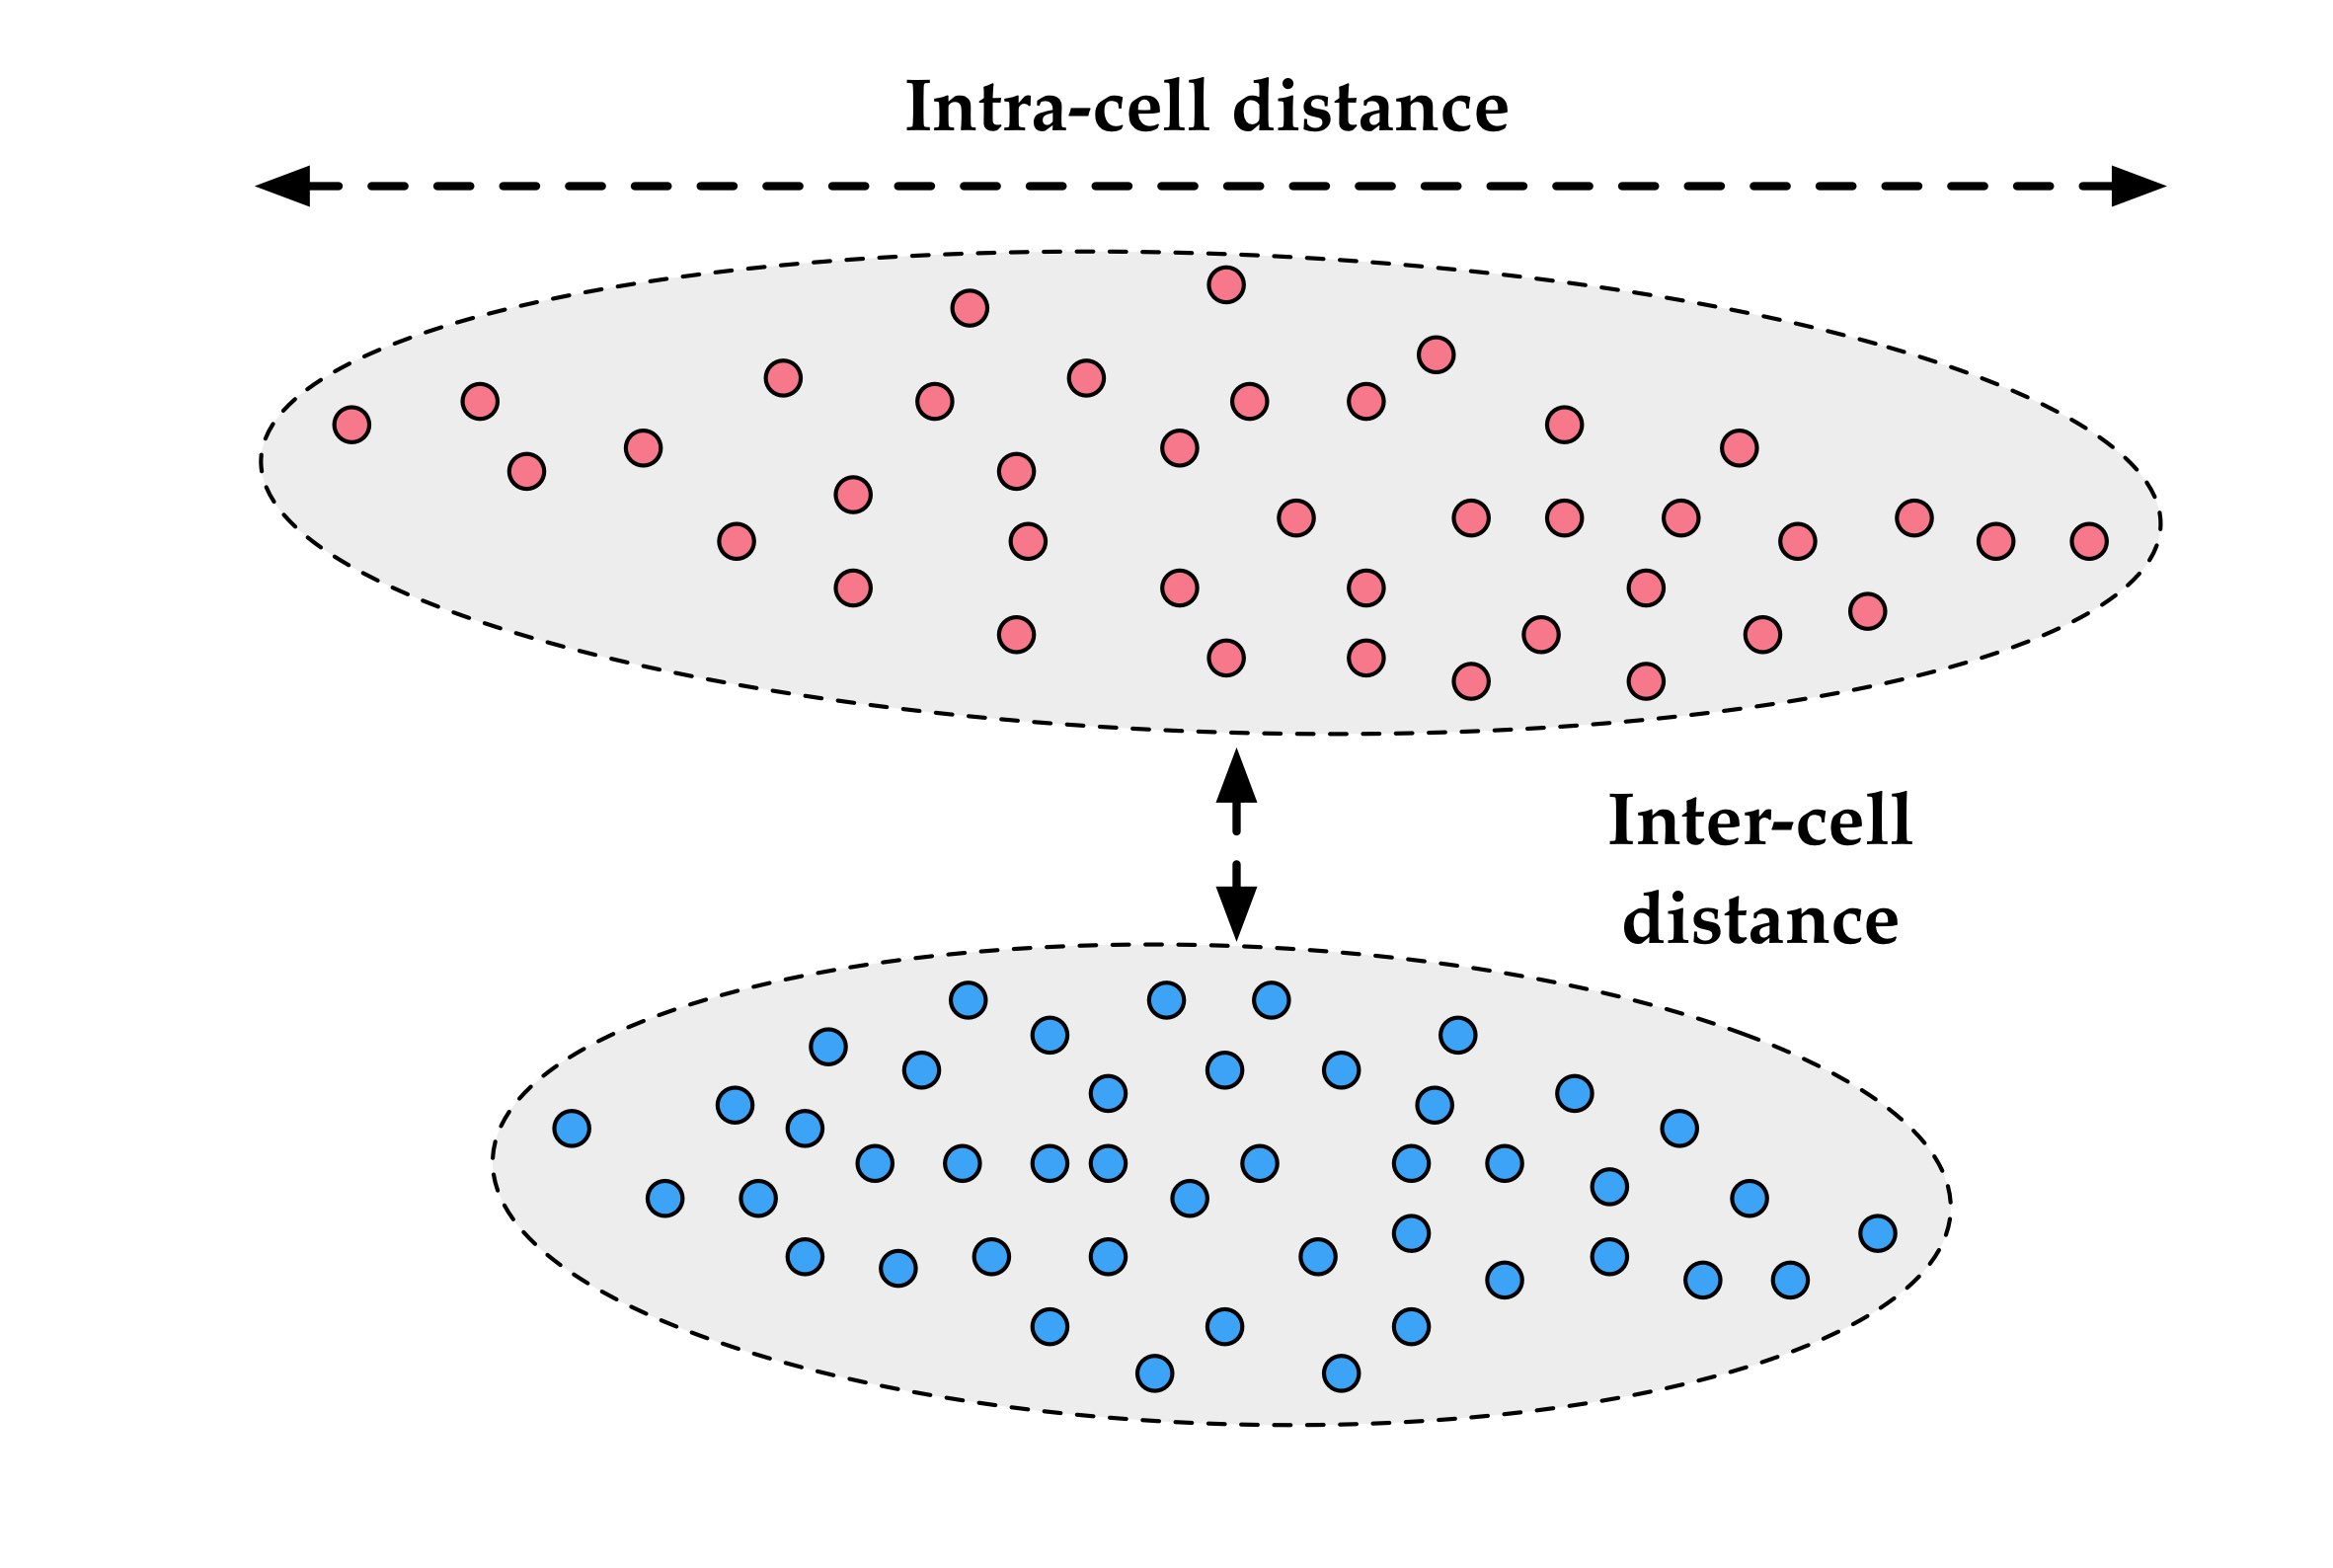
\includegraphics[width=0.5\linewidth]{Diffusion_distance.jpg}
		\caption{Example of the inefficiency of euclidean distance.}
		\label{Fig:Diffusion}
	\end{center}
\end{figure}
 
 

As $M$ is adjoint to a symmetric matrix, it is diagonizable and has a set of $n$ ordered real eigenvalues $\{\lambda_{i}\}_{j=1}^{n}$ with corresponding eigenvector $\{\psi_{i}\}_{j=1}^{n}$ . Using the $k$ first eigenvectors, a new  space can be defined for each point $i$, called the diffusion map at a given time $t$,  :
\begin{equation}
\Psi_{t}(i) = (\lambda_{2}^{t}\psi_{2}(i),\lambda_{3}^{t}\psi_{3}(i),..,\lambda_{k}^{t}\psi_{k}(i));
\end{equation}
It is possible to show that the euclidean distance in this space is a correct approximation of the diffusion distance in the initial space \citep{nadler_diffusion_2005}. We can therefore compute the location of the points in the diffusion map space and perform clustering in it using a simple k-means algorithm similarly to the NJW algorithm \citep{ng_spectral_2001,zelnik-manor_self-tuning_2004}.
In practice the choice of the number of eigenvalues used ($k$ parameter) as well as the number of clusters is made by looking for the spectral gap, i.e a significant decrease in the eigenvalues. We therefore define $k$ as being :
\begin{equation}
k = \underset{i}{ \text{argmax}}(\{\frac{\lambda_{i+1}}{\lambda_{i}}\}_{i=2}^{N_{comp}})
\end{equation}
 Here $N_{comp}$ corresponds to the maximal number of eigenvalues computed, which is equivalent to the maximal number of cells expected.
 
 The resulting clusters are then filtered using two different criteria :
 \begin{enumerate}
 \item The number of spots belonging to the cluster : clusters with less than $N_{\text{Min spots}}$ are removed. $N_{\text{Min spots}}$ is usually set to 15 to get significant clusters.
 \item The spot density of the clustering : for each cluster the two-dimensional convex hull area $A$ is computed. If the global point density is equal to $\lambda$, then by random the number of points in the convex hull will  follow a Poisson law of parameter $\lambda A$. We only select clusters where the probability of getting the observed number of spots according to the Poisson model is lower than 0.0001.
\end{enumerate}  
 
Our clustering procedure therefore results in a list of high quality clusters for each gene at each position. 
 
\subsubsection{Aggregation of spot clusters}

The obtained clusters are then gathered across the different measured genes and their potential overlap computed. To do so, a two-dimensional histogram density estimate of each cluster points is performed with .... x ... grid matrix. For each pair of clusters $i$ and $j$ with associated density estimates $p_{i}(x,y)$ and $p_{j}(x,y)$, we compute the Bhattacharyya similarity coefficient :
\begin{equation}
D_{B}(p_{i},p_{j}) = \sum_{x} \sum_{y} \sqrt{p_{i}(x,y)p_{j}(x,y)}
\end{equation}
As this coefficient is bounded between 0 (no overlap) and 1 (identical distributions), it is easy to define a global similarity threshold $\alpha$, above which two spot clusters are considered as similar. We therefore defined a squared matrix $G$, of size $|N_{cluster}N_{cluster}|$ where :

		\begin{equation}
		G_{ij} = 
		\begin{cases}
		1 & \text{if $D_{B}(p_{i},p_{j}) \geq \alpha$}\\
		0 & \text{if $D_{B}(p_{i},p_{j}) < \alpha$}\\		
		\end{cases}
		\end{equation}

A graph is then constructed using $G$ as an adjacency matrix. The connected components,  of the graph are then extracted and are considered as corresponding to a unique cell.
While the choice of the $\alpha$ parameter is left to the user, we observed in practice that a threshold value of 0.3 was stringent enough to avoid the merge of spot clusters coming from different cells.

\subsubsection{Final cell shape estimation}

The last step of our method consists in estimating the shape of the cell. To do so, for each cluster aggregate previously identified, we collect all the RNA spots across all genes. The two-dimensional density distribution of those spots is then estimated using a gaussian kernel density estimator with a bandwidth parameter $\sigma_{Spread}$. The resulting density estimate matrix is then binarized using Otsu's method and the biggest connected component is considered as the final shape of the cell.

\subsubsection{Removing cell overlaps}

While our segmentation strategy produces a good quality cell segmentation, it may generates overlapping cell areas. To remove those overlaps, we developed a heuristic algorithm that starts from a list of cell areas which partially overlap and returns a list of corrected cell areas that do not overlap. 
Let be $L_{\text{overlap}}$ the list of overlaps, i.e the list of pairs of cells sharing at least one pixel, $N_{\text{overlaps}}$ the number of overlaps, $N_{cells}$ the number of cells, and for each cell $i$, $C_{i}$ the list of pixels within its borders. Then we apply the following algorithm :

 
%bla 
 
\begin{algorithm}[H]
\DontPrintSemicolon
\SetAlgoLined
\SetKwInOut{Input}{Input}\SetKwInOut{Output}{Output}
\Input{List of overlapping cell areas $\{ C_{i}\}_{i=1}^{N_{cells}}$}
\Output{List of updated overlapping cell areas $\{ C_{i}\}_{i=1}^{N_{cells}}$}
\BlankLine
 
\For{$k = 1 \to N_{\text{overlaps}}$}{
	$i = L_{k}(1)$\;
	$j = L_{k}(2)$\;
    \eIf{$C_{i} \cap C_{j} \neq \emptyset$ }{
        $D_{i} = \frac{\text{Dist}_{\text{transform}}(C_{i})}{|C_{i}|}$\;
        $D_{j} = \frac{\text{Dist}_{\text{transform}}(C_{j})}{|C_{j}|}$\;
        $I  = C_{i} \cap C_{j} $\;
        $N_{\text{shared pixels}} = |I| $\;
        \For {$l = 1 \to N_{\text{shared pixels}}$} {
        $s = \text{argmin}(D_{i}(l),D_{j}(l))$\;
        $C_{s} = C_{s} - \{I(l)\}$
        }
    }{
    }
}
 
\caption{Cell overlap cleaning algorithm}
\end{algorithm}

\section{Image alignment and stitching}

\subsection{Requirement of Image alignment and stitching for seqFISH data processing and analysis}

During seqFISH data generation, the same positions are imaged several times to increase the number of observed genes in a linear (serial hybridization) or exponential manner (barcoding hybridization) \citep{chen_spatially_2015}. While in theory the images coming from the same position should be perfectly aligned, a significant drift can be observed primarily due to temperature variations and external vibrations. It is therefore necessary to computationally re-align the pictures before running any analysis, especially in the case of barcoding hybridization where the same RNA spot has to be identified across the different rounds to perform demultiplexing.

A similar procedure has to be applied to perform image stitching, that is to say to combine multiple images with overlapping fields of view to produce a panoramic picture. Indeed it is possible to automatically image a whole tissue section by generating partially overlapping images (usually around 10 to 20 \% of overlap). While the theoretical overlap between pictures is known, it can vary in practice and need to be precisely estimated in an automated manner.

Both problems are linked and are part of what is known as Image Registration. The following subsections will describe the computational method used to solve both problems as well as its implementation and practical details.


\subsection{Image registration using phase correlation method}

Over the last decades several methods have been developed to align or stitch related images. As we do not aim to provide an exhaustive review of the field, we recommend the interested readers to have a look at the excellent review by Szeliski \citep{szeliski_image_2006}. 

We decided to use the Fourrier transform based Phase correlation method, a method commonly used for microscopy image stitching \citep{szeliski_image_2006,preibisch_globally_2009} due to its high efficiency and low computational cost thanks to Fast Fourrier Transform (FFT). While this image registration method is only able to deal with translation-based alignment, we considered that rotation and scaling transformation where not likely to happen in our experimental setting. 

Let $g_{A}$ and $g_{B}$ be two different images of same size ($N \times M$). Let $G_{a} = F(g_{A})$ and $G_{b} = F(g_{B})$ their respective discrete Fourrier transform signal. We can compute the cross-power spectrum  R matrix :

\begin{equation}
R = \frac{G_{a} \odot \overline{G_{b}}}{|G_{a} \odot \overline{G_{b}}|}
\label{eq:Cross_power_spectrum}
\end{equation}

where $\odot$ corresponds to the Hadamard product (element wise matrix multiplication) and  $\overline{G_{b}}$ the complex conjugate of ${G_{b}}$.  The inverse Fourrier transform of R can then be obtained and used to identify the translation vector $v$ :

\begin{equation}
r = F^{-1}(R)
\end{equation}

\begin{equation}
(v_{x},v_{y}) = \text{argmax}(r)
\end{equation}

This technique is motivated by the shifting property of Fourrier transform. Indeed if image $g_{B}$ is generated from perfect (cyclic) shift of image $g_{A}$, i.e  $g_{B}(x,y) = g_{A}(x+v_{x},y+v_{y})$, then :

\begin{equation}
 G_{b}(w,z) = e^{-2\pi j (\frac{w v_{x} }{N}+ \frac{z v_{y} }{M})}G_{a}(w,z)
\end{equation}

We can then simplify equation  \ref{eq:Cross_power_spectrum}.

\begin{equation}
R(w,z) = e^{-2\pi j (\frac{w v_{x} }{N}+ \frac{z v_{y} }{M})}
\end{equation}
The inverse Fourrier transform of R will therefore result in a highly localized peak corresponding to the shift vector.


In practice, to increase the performance of the phase correlation method, we applied a filter to increase the signal from the borders in the case of image stitching . This two dimensional filter, $H$, correspond to one minus the Hamming filter :

\begin{equation}
H(x,y) = (1 -  \frac{1}{2} (1-cos(2 \pi \frac{x}{N_{x}}))) (1 -  \frac{1}{2} (1-cos(2 \pi \frac{y}{N_{y}})))
\end{equation}

where $N_{x}$ and $N_{y}$ to the $x$ and $y$ size values.

\begin{figure}[!h]
	\begin{center}
	
		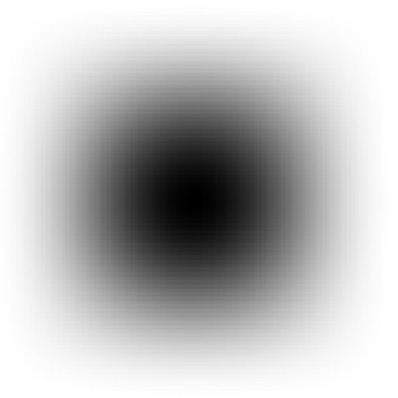
\includegraphics[width=0.5\linewidth]{Hanning_inverse.jpg}
		\caption{Inverse two-dimensional Hanning filter function.}
		\label{Fig:Diffusion}
	\end{center}
\end{figure}

Conversely, in the case of image alignment, a classical Hanning filter is used.

\subsection{Computation of the cumulative stitching vectors }

Stitching more than two images together is a challenging task, as independent pairwise transforms may not agree when the image share several neighbors. To overcome this limitation we developed a  graph based method that blindly identifies and favors robust stitching vectors.

Lets consider a set of  $N_{\text{Image}}$ overlapping images. We assume that each image overlaps with at least one other image. First, the phase correlation method is applied for each possible pair of non identical images. To quantify the likelihood that the two images, $i$ and $j$, are indeed overlapping, the ratio between the maximal value of the phase correlation matrix $r_{ij}$ (correlation peak height) and the standard variation of $r_{ij}$ values is computed :

\begin{equation}
		S_{ij}  = 
		\begin{cases}
		\frac{\max(r_{i,j})}{\sigma(r_{i,j)}} & \text{if $i \neq j $}\\
		0 & \text{if $i=j$}\\		
		\end{cases}
\end{equation}

We therefore end up with a symmetric matrix of size $|N_{\text{Image}}|$.  This matrix value must then be thresholded to identify significant and non significant stitching vectors. To do so we applied Otsu's thresholding on the non null elements of the matrix to obtain a threshold $T$. A thresholded version of $S$, $S^{\text{threshold}}$  is then computed :

\begin{equation}
		S_{ij}^{\text{Threshold}}  = 
		\begin{cases}
		1 & \text{if $S_{ij} \geq T $}\\
		0 & \text{if $S_{ij} < T$}\\		
		\end{cases}
\end{equation}

An undirected graph $G$ is then build using $S^{\text{Threshold}}$ as adjacency matrix.

 While automated thresholding is usually performing well, we established a list of criterion to control for the value of T based on the obtained graph $G$. Indeed, if the graph is interpreted as a representation of the overlaps between pictures (nodes correspond to images and edges to significant overlap), then the graph should respect the following rules :

\begin{itemize}
\item Only one connected component of size strictly bigger than one should be observed in $G$.
\item There must be at least  $N_{\text{Image}} - 1$ edges in $G$.
\item If we consider that the images are spread on a regular grid then the maximal number of edges in $G$ is equal to $2(N_{\text{Image}}-\sqrt{N_{\text{Image}}})$.  
\end{itemize}

Therefore an upper ($T_{max}$) and lower bounds ($T_{min}$) of $T$ can computed with $T_{max}$ being equal to the $N_{\text{Image}} - 1$ highest value of $S$ and $T_{min}$ to the $2(N_{\text{Image}}-\sqrt{N_{\text{Image}}})$ highest value of $S$. Thus, even before $G$ is computed, $T$ is updated :

\begin{equation}
		T_{\text{updated}} = 
		\begin{cases}
		T_{max} & \text{if $T \geq T_{max} $}\\
		T_{min} & \text{if $T \leq T_{min}$}\\		
		T & \text{if $T_{min} < T < T_{max}  $} \\
		\end{cases}
\end{equation}

The graph $G$ is then computed and evaluated : if only one connected component with strictly more than one node  is observed then the graph is used as is. However if multiple connected components are observed then the threshold value is progressively lowered and the graph build until a unique connected component is observed. If no connected component is observed while T has reached $T_{min}$, then the stitching procedure is stopped and an error message provided.

 
\begin{figure}[!h]
	\begin{center}
		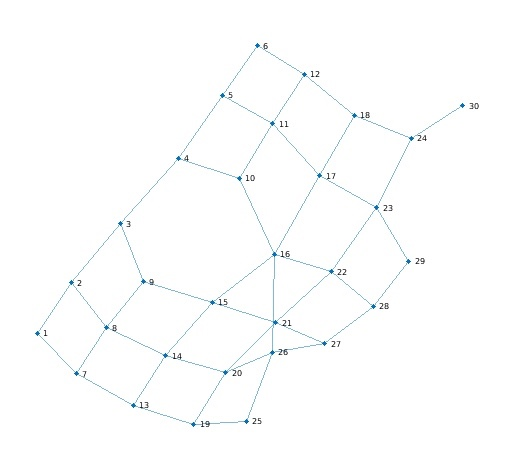
\includegraphics[width=0.8\linewidth]{Graph_stitching.jpeg}
		\caption{Example of a stitching graph from 30 images placed on a rectangular grid}
		\label{Fig:Graph_stitching}
	\end{center}
\end{figure}


Once the graph is build, a reference image is chosen and the shortest graph path between each node and the node corresponding to the reference image are computed. These paths are then used to compute the final stitching vectors. Let $p_{i}$ be a path between the node $i$ and the reference node, that is to say a collection of edges allowing to go from node $i$ to the reference node, then the final stitching vector for image $i$ is equal to the sum of each stitching vectors corresponding to the edges in that path:

\bibliographystyle{unsrt}
\bibliography{Biblio_seqFISH_math}


\end{document}
